\section{Resultados obtenidos}
\label{sec:resultados}

Todos los valores reportados en esta sección provienen de la ejecución del
módulo con la parametrización de la tabla~\ref{tab:parametros} y semilla
\num{42}, y son reproducibles ejecutando el código del anexo digital.

\subsection{Reconstrucción del volumen de carga}

La tabla~\ref{tab:resultados-volumen} presenta las métricas de error sobre la
variable observada, promediadas sobre las $M = 50$ corridas independientes.

\begin{table}[H]
\centering
\caption{Métricas de error en la reconstrucción del volumen de carga
($M = 50$ corridas, $N = 1000$ pasos).}
\label{tab:resultados-volumen}
\footnotesize
\begin{tabular}{@{}lS[table-format=1.4]S[table-format=1.4]S[table-format=2.2]@{}}
\toprule
\textbf{Métrica} & {\textbf{SCADA crudo}} & {\textbf{Filtro de Kalman}} &
{\textbf{Reducción [\si{\percent}]}}\\
\midrule
MSE [\si{\metre\tothe{6}}]  & 4.9660 & 0.5179 & 89.57\\
Desviación del MSE          & 0.2340 & 0.0865 & {---}\\
RMSE [\si{\metre\cubed}]    & 2.2278 & 0.7173 & 67.80\\
Desviación del RMSE         & 0.0522 & 0.0588 & {---}\\
\bottomrule
\end{tabular}
\end{table}

El error cuadrático medio de la telemetría cruda, \SI{4,97}{\metre\tothe{6}},
coincide con la varianza de ruido inyectada $R = \SI{5,0}{\metre\tothe{6}}$,
como corresponde por construcción, lo que constituye una verificación interna de
la correcta implementación del generador de degradación.

La figura~\ref{fig:reconstruccion} muestra la reconstrucción de la trayectoria
en una corrida representativa. El perfil en diente de sierra corresponde al
ciclo operacional real: descarga discontinua de camiones sobre extracción
continua del chancador.

\begin{figure}[H]
\centering
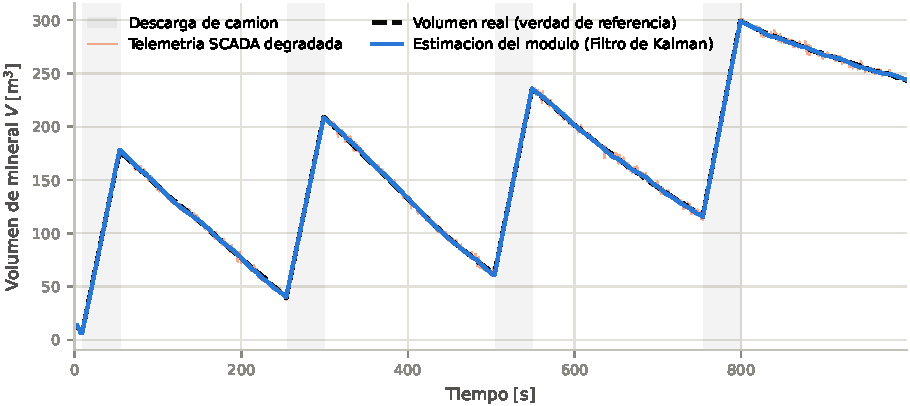
\includegraphics[width=\textwidth]{figuras/fig1_reconstruccion_volumen.pdf}
\caption{Reconstrucción dinámica del volumen de carga en la tolva de recepción.
Las bandas sombreadas indican los eventos de descarga de camión.}
\label{fig:reconstruccion}
\end{figure}

\subsection{Reconstrucción de la variable latente}

El resultado de mayor relevancia conceptual corresponde a la tasa de llenado
$\dot{V}_{k}$, variable que no cuenta con instrumentación alguna.

\begin{table}[H]
\centering
\caption{Métricas de error en la reconstrucción de la tasa de llenado, variable
no sensada.}
\label{tab:resultados-tasa}
\footnotesize
\begin{tabular}{@{}lS[table-format=1.4]S[table-format=1.4]S[table-format=2.2]@{}}
\toprule
\textbf{Métrica} & {\textbf{Diferencias finitas}} &
{\textbf{Filtro de Kalman}} & {\textbf{Reducción [\si{\percent}]}}\\
\midrule
RMSE [\si{\metre\cubed\per\second}] & 3.6891 & 0.0674 & 98.17\\
\bottomrule
\end{tabular}
\end{table}

La magnitud de la diferencia merece atención. La línea base disponible para un
sistema SCADA convencional —derivar numéricamente la señal cruda— produce un
error de \SI{3,69}{\metre\cubed\per\second} sobre una magnitud física cuyo valor
nominal es \SI{0,8}{\metre\cubed\per\second}: el procedimiento entrega ruido y
no información. El módulo reduce ese error a
\SI{0,067}{\metre\cubed\per\second}, lo que representa una mejora del
\SI{98,17}{\percent}. La figura~\ref{fig:latente} contrasta ambos
procedimientos.

\begin{figure}[H]
\centering
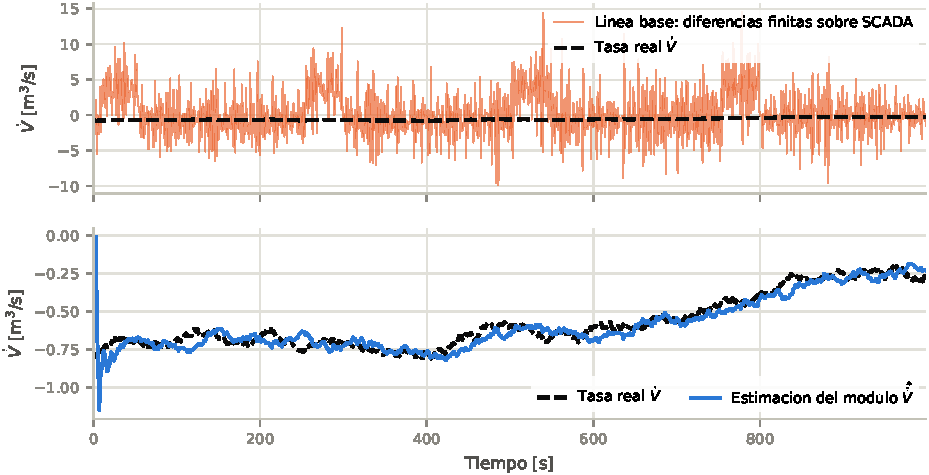
\includegraphics[width=\textwidth]{figuras/fig2_tasa_latente.pdf}
\caption{Recuperación de la variable latente. Panel superior: línea base por
diferencias finitas sobre la señal cruda. Panel inferior: estimación del módulo,
en escala física. Nótese la diferencia de escala entre ambos paneles.}
\label{fig:latente}
\end{figure}

\subsection{Convergencia asintótica del estimador}

La figura~\ref{fig:convergencia} evidencia la convergencia de la covarianza del
error y de la ganancia de Kalman hacia sus valores de régimen permanente,
comportamiento predicho por la formulación de Riccati para sistemas lineales
invariantes \parencite{simon2006}. La convergencia se alcanza en torno a los
\SI{60}{\second} de operación, con $K_{1} \to \num{0,0993}$.

\begin{figure}[H]
\centering
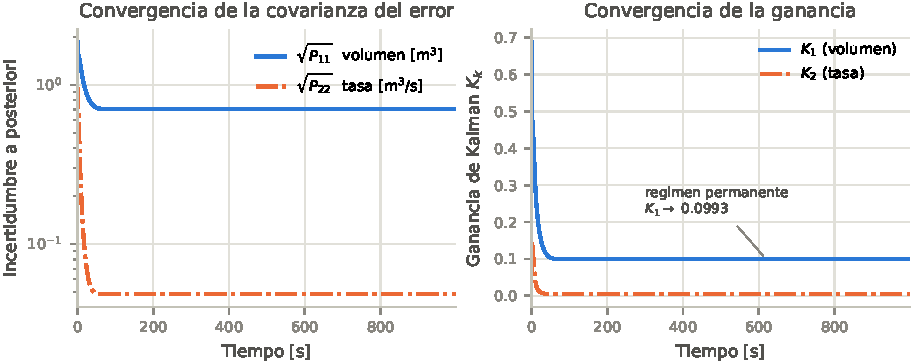
\includegraphics[width=\textwidth]{figuras/fig3_convergencia.pdf}
\caption{Convergencia asintótica de la covarianza del error de estimación y de
la ganancia de Kalman hacia el régimen permanente.}
\label{fig:convergencia}
\end{figure}

\subsection{Validación estadística}

La tabla~\ref{tab:inferencia} reporta la inferencia sobre el RMSE, expresada en
\si{\metre\cubed}.

\begin{table}[H]
\centering
\caption{Inferencia estadística pareada sobre el RMSE del volumen
($M = 50$; $\alpha = 0{,}05$).}
\label{tab:inferencia}
\footnotesize
\begin{tabular}{@{}ll@{}}
\toprule
\textbf{Estadístico} & \textbf{Valor}\\
\midrule
Reducción media del RMSE & \SI{1,5106}{\metre\cubed}\\
Intervalo de confianza al \SI{95}{\percent} &
$[1{,}4881;\ 1{,}5330]$~\si{\metre\cubed}\\
Prueba t pareada (unilateral) & $t(49) = 135{,}24$; $p = 5{,}15\times10^{-65}$\\
Tamaño del efecto ($d$ de Cohen) & \num{19,13}\\
Normalidad (Shapiro-Wilk) & $W = 0{,}9459$; $p = 0{,}0233$ \quad
\textbf{(se rechaza)}\\
Contraste robusto (Wilcoxon) & $W = 1275{,}0$; $p = 8{,}88\times10^{-16}$\\
Decisión & Se rechaza $H_{0}$\\
\bottomrule
\end{tabular}
\end{table}

Corresponde detenerse en el resultado de la verificación de normalidad. La
prueba de Shapiro-Wilk \textbf{rechaza} el supuesto de normalidad de las
diferencias ($p = 0{,}0233 < 0{,}05$), de modo que la aplicación mecánica de la
prueba t sería, en rigor, cuestionable. Es precisamente por esta razón que el
diseño incorporó el contraste no paramétrico de Wilcoxon, que no exige
normalidad y que confirma la conclusión con
$p = 8{,}88\times10^{-16}$. La coincidencia de ambas pruebas permite sostener el
rechazo de $H_{0}$ con independencia del supuesto paramétrico. Debe añadirse que
con $M = 50$ observaciones el teorema central del límite otorga a la prueba t
una robustez considerable frente a desviaciones moderadas de la normalidad, y
que la magnitud del efecto —una $d$ de Cohen de \num{19,13}, más de un orden de
magnitud por sobre el umbral convencional de efecto grande— hace que ninguna
consideración distribucional pueda revertir la conclusión.

Sobre la variable latente, la inferencia arroja $t(49) = 296{,}36$ con
$p = 1{,}09\times10^{-81}$ e intervalo de confianza al \SI{95}{\percent} de
$[3{,}5971;\ 3{,}6463]$~\si{\metre\cubed\per\second}.

\begin{figure}[H]
\centering
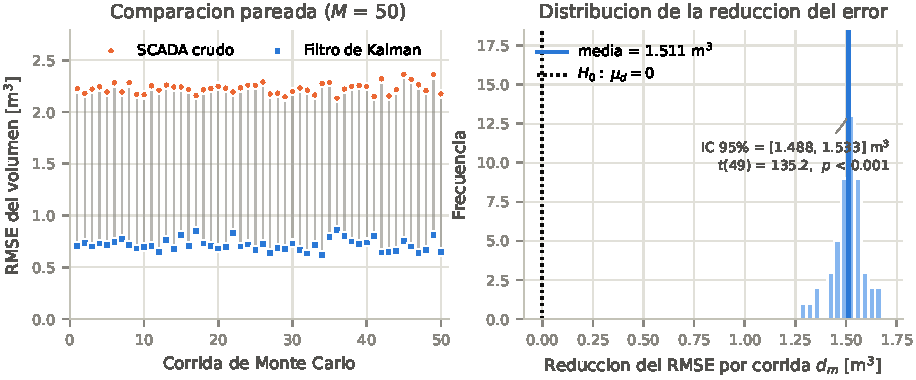
\includegraphics[width=\textwidth]{figuras/fig4_montecarlo.pdf}
\caption{Validación de Monte Carlo. Panel izquierdo: comparación pareada corrida
a corrida. Panel derecho: distribución de la reducción del RMSE, con la
hipótesis nula señalada en el origen.}
\label{fig:montecarlo}
\end{figure}

\subsection{Sensibilidad ante la degradación del entorno}

La tabla~\ref{tab:degradacion} y la figura~\ref{fig:degradacion} muestran el
comportamiento del módulo ante niveles crecientes de ruido real del sensor.

\begin{table}[H]
\centering
\caption{Desempeño del módulo ante niveles crecientes de degradación
instrumental.}
\label{tab:degradacion}
\footnotesize
\begin{tabular}{@{}S[table-format=3.0]S[table-format=2.2]S[table-format=3.3]S[table-format=2.3]S[table-format=2.2]@{}}
\toprule
{$R$ [\si{\metre\tothe{6}}]} & {$\sigma_{v}$ [\si{\metre\cubed}]} &
{MSE SCADA [\si{\metre\tothe{6}}]} & {MSE KF [\si{\metre\tothe{6}}]} &
{Reducción [\si{\percent}]}\\
\midrule
1   & 1.00  & 0.987   & 0.165  & 83.32\\
5   & 2.24  & 4.937   & 0.527  & 89.33\\
20  & 4.47  & 19.748  & 1.449  & 92.66\\
50  & 7.07  & 49.369  & 2.831  & 94.27\\
100 & 10.00 & 98.738  & 4.707  & 95.23\\
200 & 14.14 & 197.476 & 7.843  & 96.03\\
400 & 20.00 & 394.953 & 13.093 & 96.68\\
\bottomrule
\end{tabular}
\end{table}

La reducción del error crece de forma monótona con la severidad de la
degradación, desde el \SI{83,32}{\percent} en condiciones benignas hasta el
\SI{96,68}{\percent} en degradación extrema. El aporte del módulo, por tanto, no
se diluye en entornos hostiles sino que se acentúa.

\begin{figure}[H]
\centering
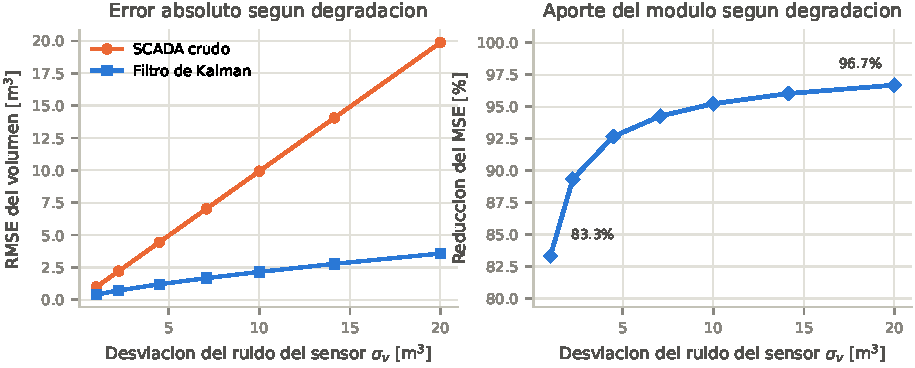
\includegraphics[width=\textwidth]{figuras/fig5_degradacion.pdf}
\caption{Comportamiento del módulo ante niveles crecientes de ruido
instrumental. Izquierda: error absoluto de ambas fuentes. Derecha: reducción
relativa del MSE.}
\label{fig:degradacion}
\end{figure}

\subsection{Robustez ante desajuste de sintonización}

La figura~\ref{fig:sensibilidad} presenta la malla de RMSE resultante de
desajustar intencionalmente las covarianzas del filtro respecto de la física
real.

\begin{figure}[H]
\centering
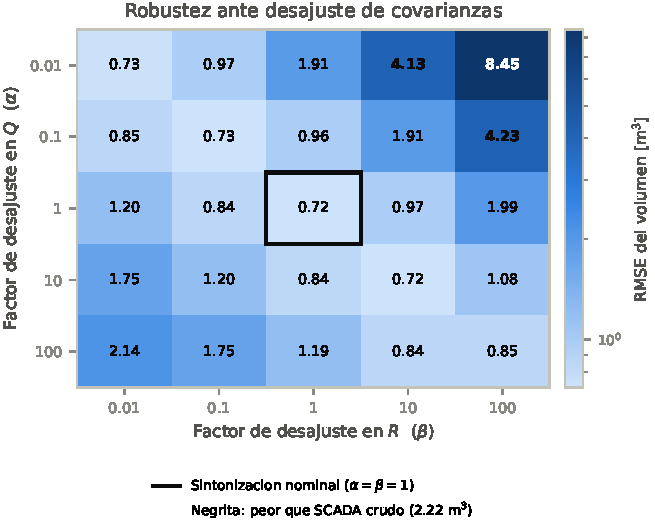
\includegraphics[width=0.82\textwidth]{figuras/fig6_sensibilidad_QR.pdf}
\caption{Robustez del módulo ante desajuste intencional de las covarianzas
$\mathbf{Q}$ y $\mathbf{R}$. El recuadro señala la sintonización nominal.}
\label{fig:sensibilidad}
\end{figure}

El resultado presenta una estructura diagonal marcada. Con sintonización nominal
el RMSE es \SI{0,721}{\metre\cubed}, frente a \SI{2,224}{\metre\cubed} de la
telemetría cruda. A lo largo de la diagonal —donde ambas covarianzas están
escaladas por el mismo factor, incluso hasta cien veces en cualquier dirección—
el desempeño se mantiene en el rango \SIrange{0,72}{0,85}{\metre\cubed}, muy
cerca del óptimo. La degradación severa aparece solo en las esquinas
antidiagonales, y el peor caso de la malla alcanza \SI{8,45}{\metre\cubed}.

De las veinticinco combinaciones evaluadas, únicamente tres resultan peores que
no filtrar. Este hallazgo tiene una lectura de ingeniería directa: lo que
gobierna el desempeño del estimador es la \emph{razón} $\mathbf{Q}/\mathbf{R}$ y
no los valores absolutos de ambas matrices, resultado consistente con la teoría
de estimación óptima y de considerable valor práctico, puesto que implica que un
error de calibración proporcional en ambas covarianzas es esencialmente
inofensivo.

\subsection{Verificación de reproducibilidad}

Dos ejecuciones sucesivas e independientes del experimento produjeron archivos
de salida idénticos byte a byte, verificado mediante suma de verificación MD5
sobre los cuatro registros CSV generados. La reproducibilidad exacta del estudio
es, por tanto, un hecho comprobado y no una declaración de intención.

\subsection{Extensibilidad del núcleo del módulo}
\label{sec:extensibilidad}

Como evidencia complementaria del carácter desacoplado del módulo, el mismo
núcleo del estimador se aplicó sin modificación alguna de su código a otros tres
subsistemas del activo: la dinámica electromecánica de potencia activa del motor
principal, la dinámica térmica del estator y la tendencia de desgaste
estructural del revestimiento. En los tres casos únicamente se sustituyen las
matrices del sistema que se entregan al constructor de la clase.

Este resultado no forma parte de la validación central del estudio, cuyo objeto
declarado es el volumen de tolva, pero acredita empíricamente la propiedad de
autocontención y desacoplamiento comprometida en el alcance del proyecto, y
sugiere una vía de extensión natural que se recoge en las proyecciones de la
sección~\ref{sec:conclusiones}.
